% TODO: Falar que utilizamos o hit rate para ver se nossos modelos eram capazes de pelo menos prever quando que vai diminuir e quando que vai aumentar

% TODO?: Adicionar gráfico que mostra o tempo de predição

Este capítulo tem como objetivo apresentar uma discussão acerca dos resultados dos experimentos. Primeiramente, será exposto o ambiente de experimento serão discutidos como os modelos reagem à variação dos principais parâmetros, quantidade de divisões, passado visível e tamanho do intervalo do fluxo. Subsequentemente, serão apresentados os resultados de como os modelos reagem para a escolha dos hiper-parâmetros selecionados. Por fim, serão analisados os resultados das previsões de fluxo de cada modelo nos curtos prazos de 15, 30, 45 e 60 minutos.


\section{Ambiente de Experimento}

O ambiente de experimento foi um servidor equipado com Ubuntu 64 bits. O servidor possui dois CPUs \textit{Intel(R) Xeon(R) Platinum 8160 CPU @ 2.10GHz} e 251 GiB de memória principal. Cada CPU dessas possui 24 núcleos e executa até 48 \textit{threads} em paralelo. No total então são 96 \textit{threads}, que foram usados paralelamente para acelerar a execução do experimento. Porém, em algumas partes da execução, menos \textit{threads} tiveram que ser usadas, pois não havia memória principal o suficiente para todas as instâncias em paralelo.

\section{Resultados das Escolhas de Parâmetros}
\label{section:resultados_parametros}

Após o tratamento dos dados, foram realizados diversos testes para definir os melhores parâmetros de cada modelo. Devido a limitações de hardware os parâmetros foram considerados independentes. Ou seja, cada um deles possui um valor padrão e será analisado como esse parâmetro se comporta dado a fixação dos outros. Além disso, as otimizações estão sendo feitas no pior caso da predição, isto é, na predição de 1h no futuro. Na lista abaixo podem ser vistos os parâmetro que foram levados em consideração nos estudos de caso deste trabalho.

\begin{enumerate}
	\item \textbf{Número de divisões do conjunto de dados} (\textit{Blocking}): Número de divisões utilizadas no blocking para criar mais subconjuntos de dados. Os valores testados foram: 1,2,4,8. Para cada subconjunto, a porcentagem utilizada para treinamento e teste foi a mesma: 80\% para treinamento e 20\% para testes. O valor padrão utilizado foi de 4 divisões.
	\item \textbf{Passado Visível}: Parâmetro que define qual a janela de tempo no passado que será visível no treinamento do modelo. O valor inicial considerado foi de 480 minutos. Os valores de 60, 120, 240 e 480 minutos também foram testados.
	\item \textbf{Tamanho do intervalo do fluxo}: Parâmetro que define o intervalo de tempo no qual será acumulado a quantidade de veículos para o cálculo do fluxo. O valor inicial de teste foi 2,5 minutos. Foram realizados testes para as variações de 5 e 7,5 minutos também (ou 150, 300 e 450 segundos).
\end{enumerate}

\subsection{Número de Divisões do Conjunto de Dados}

Na Figura \ref{figure:res_split} pode ser observado que todos os modelos apresentaram uma performance melhor que as bases de comparação. Os resultados também são um indicativo que não é necessário um tamanho muito grande de treino para que os modelos se ajustem a distribuição do conjunto de dados. No caso, o melhor número de divisão do conjunto de dados para a maioria os modelos foi  8, como pode ser observado na Tabela \ref{table:res_split}. Como o tamanho do conjunto de dados é de 52.992 (intervalo de fluxo padrão foi de 150 segundos), os modelos foram capazes de se ajustar com apenas 5300 dados (aproximadamente), o que seria equivalente a um pouco mais de 1 semana. Os únicos modelos que não apresentaram os melhores resultados com o número de divisões igual a 8 foram \textit{\acrshort{SVM}} e \textit{\acrshort{GRU}} que utilizaram a versão A do conjunto de dados. Porém, mesmo estes modelos tiveram diferenças pouco significativas se comparados com os seus resultado de 8 divisões. Vale notar também que a maioria dos modelos apresentou uma piora nas predições quando fora utilizado 4 como número de divisão, o que seria equivalente a duas semanas.

\begin{figure}[htbp]
    \centering
    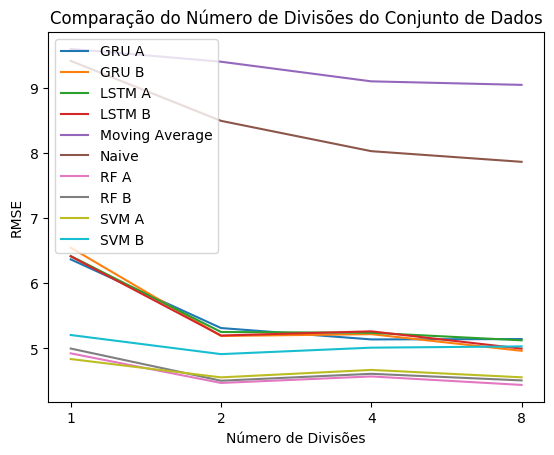
\includegraphics[scale=0.8]{monography/img/comparisons/comparacao_do_numero_de_divisoes_do_conjunto_de_dados_rmse.png}
    \label{figure:res_split}
    \caption[Resposta dos modelos à variação do número de divisões do conjunto de dados]{Resposta dos modelos à variação do número de divisões do conjunto de dados}
\end{figure} 

\begin{table}[htbp]
    \begin{tabular*}{\linewidth}{@{\extracolsep{\fill}}lllll}
    \toprule
     & 
    \multicolumn{1}{l}{\textbf{1}} & 
    \multicolumn{1}{l}{\textbf{2}} &
    \multicolumn{1}{l}{\textbf{4}} &
    \multicolumn{1}{l}{\textbf{8}} \\
    \midrule
    \textbf{MM} & 9.596 $\pm$ 0.000 & 9.399 $\pm$ 0.008 & 9.098 $\pm$ 0.740 & \textbf{9.044} $\pm$ 0.881
    \\
    \midrule
    \textbf{Naive} & 9.413 $\pm$ 0.000 & 8.492 $\pm$ 0.777 & 8.026 $\pm$ 0.868 & \textbf{7.863} $\pm$ 0.889
    \\
    \midrule
    \textbf{RF A} & 4.924 $\pm$ 0.000 & 4.469 $\pm$ 0.254 & 4.569 $\pm$ 0.739 & \textbf{4.439} $\pm$ 0.513
    \\
    \midrule
    \textbf{RF B} & 4.997 $\pm$ 0.000 & 4.504 $\pm$ 0.240 & 4.610 $\pm$ 0.745 & \textbf{4.508} $\pm$ 0.501
    \\
    \midrule
    \textbf{SVM A} & 4.836 $\pm$ 0.000 & \textbf{4.555} $\pm$ 0.160 & 4.669 $\pm$ 0.736 & 4.556 $\pm$ 0.494
    \\
    \midrule
    \textbf{SVM B} & 5.205 $\pm$ 0.000 & \textbf{4.912} $\pm$ 0.042 & 5.011 $\pm$ 0.618 & 5.030 $\pm$ 0.513
    \\
    \midrule
    \textbf{LSTM A} & 6.418 $\pm$ 0.000 & 5.251 $\pm$ 0.279 & 5.239 $\pm$ 0.794 & \textbf{5.123} $\pm$ 0.672
    \\
    \midrule
    \textbf{LSTM B} & 6.412 $\pm$ 0.000 & 5.197 $\pm$ 0.156 & 5.261 $\pm$ 0.830 & \textbf{4.996} $\pm$ 0.696
    \\
    \midrule
    \textbf{GRU A} & 6.366 $\pm$ 0.000 & 5.312 $\pm$ 0.014 & \textbf{5.137} $\pm$ 0.702 & 5.143 $\pm$ 0.516
    \\
    \midrule
    \textbf{GRU B} & 6.545 $\pm$ 0.000 & 5.190 $\pm$ 0.030 & 5.218 $\pm$ 0.686 & \textbf{4.963} $\pm$ 0.643
    \\
    \bottomrule
    \end{tabular*}
    \label{table:res_split}
    \caption{Resultados da Comparação entre os números de divisões. Melhores resultados de cada modelo em negrito.}
\end{table}

\subsection{Passado Visível}

% TODO: reference the seeable_past_time

A respeito da variação no quanto do passado o modelo tem acesso, é perceptível na Figura \ref{figure:res_past} que quanto mais acesso ao passado o modelo tiver, melhor será sua predição. Percebe-se também que o melhor valor para a quantidade de acesso do passado, dentre os testados, são 480 minutos (ou 8 horas). Porém, é importante ressaltar que mais acesso ao passado também implica em uma quantidade de treino maior, ou seja, maior custo computacional, especialmente para modelos de aprendizagem profunda. Dito isso, e considerando que a escala do eixo X é exponencial (Passado visível: 60, 120, 240, 480), pode-se que concluir que para conseguir resultados ainda melhores, seria necessário aumentar de maneira significativa a quantidade de passado visível, o que, talvez, não valesse o aumento do custo computacional, já que, para cada aumento exponencial do eixo X, a qualidade da predição melhora apenas de maneira linear. A respeito das bases de comparação, também é claro que o modelo \textit{Naive} não é afetado pela quantidade de tempo de passado visível, mas ainda assim há uma leve mudança no conjunto de dados, pois ao se mudar este parâmetro, o último valor recebido pelo modelo \textit{Naive} é mudado também, afetando suas predições e gerando as diferenças vistas na Tabela \ref{table:res_past}. Já o modelo \acrshort{MM} é o único que piora com o tempo. 


\begin{figure}[htbp]
    \centering
    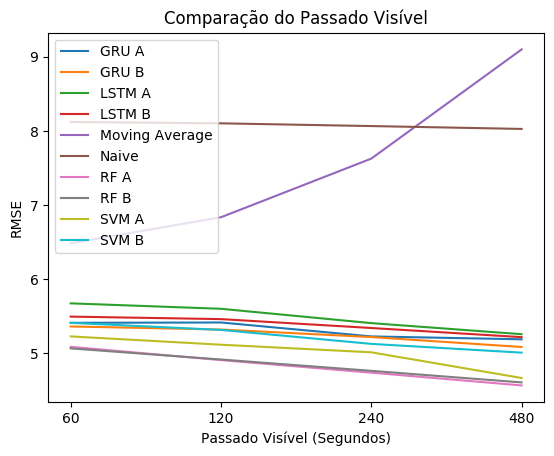
\includegraphics[scale=0.8]{monography/img/comparisons/comparacao_do_passado_visivel_rmse.png}
    \label{figure:res_past}
    \caption[Resposta dos modelos à variação dos valores de passado visível]{Resposta dos modelos à variação dos valores de passado visível}
\end{figure}
 
\begin{table}[htbp]
    \begin{tabular*}{\linewidth}{@{\extracolsep{\fill}}lllll}
    \toprule
     & 
    \multicolumn{1}{l}{\textbf{60}} & 
    \multicolumn{1}{l}{\textbf{120}} &
    \multicolumn{1}{l}{\textbf{240}} &
    \multicolumn{1}{l}{\textbf{480}} \\
    \midrule
    \textbf{MM} & \textbf{6.485} $\pm$ 0.627 & 6.836 $\pm$ 0.649 & 7.626 $\pm$ 0.684 & 9.098 $\pm$ 0.740
    \\
    \midrule
    \textbf{Naive} & 8.120 $\pm$ 0.869 & \textbf{8.102} $\pm$ 0.873 & 8.065 $\pm$ 0.887 & 8.026 $\pm$ 0.868 
    \\
    \midrule
    \textbf{RF A} & 5.089 $\pm$ 0.758 & 4.910 $\pm$ 0.735 & 4.741 $\pm$ 0.707 & \textbf{4.569} $\pm$ 0.739 
    \\
    \midrule
    \textbf{RF B} & 5.069 $\pm$ 0.753 & 4.918 $\pm$ 0.728 & 4.766 $\pm$ 0.705 & \textbf{4.610} $\pm$ 0.745 
    \\
    \midrule
    \textbf{SVM A} & 5.230 $\pm$ 0.700 & 5.118 $\pm$ 0.706 & 5.015 $\pm$ 0.691 & \textbf{4.669} $\pm$ 0.736 
    \\
    \midrule
    \textbf{SVM B} & 5.412 $\pm$ 0.627 & 5.318 $\pm$ 0.624 & 5.129 $\pm$ 0.586 & \textbf{5.011} $\pm$ 0.618 
    \\
    \midrule
    \textbf{LSTM A} & 5.675 $\pm$ 0.814 & 5.602 $\pm$ 0.713 & 5.409 $\pm$ 0.750 & \textbf{5.260} $\pm$ 0.769 
    \\
    \midrule
    \textbf{LSTM B} & 5.497 $\pm$ 0.563 & 5.463 $\pm$ 0.573 & 5.343 $\pm$ 0.731 & \textbf{5.220} $\pm$ 0.763 
    \\
    \midrule
    \textbf{GRU A} & 5.413 $\pm$ 0.702 & 5.417 $\pm$ 0.650 & 5.230 $\pm$ 0.610 & \textbf{5.191} $\pm$ 0.742 
    \\
    \midrule
    \textbf{GRU B} & 5.364 $\pm$ 0.631 & 5.322 $\pm$ 0.710 & 5.221 $\pm$ 0.747 & \textbf{5.087} $\pm$ 0.679
    \\
    \bottomrule
    \end{tabular*}
    \label{table:res_past}
    \caption{Resultados da Comparação entre as quantidade de passados visíveis. Melhores resultados de cada modelo em negrito.}
\end{table}
 
\subsection{Tamanho do Intervalo do Fluxo}

Por último, pode-se notar na Figura \ref{figure:res_flow} que o tamanho do intervalo do fluxo adotado impacta de maneira significativa a qualidade das predições dos modelos. Esse efeito pode ser justificado pela quantidade de dados resultantes de cada tamanho do intervalo de fluxo, visto que quanto maior o intervalo, menor a quantidade de dados. Por exemplo, são 52.992 dados para 2,5 minutos (150 segundos) e 17.664 para 7.5 minutos (450 segundos). O que torna mais extenso o tempo de treinamento. Dos valores testados, 2.5 minutos é o melhor tamanho de intervalo de fluxo para todos os modelo, como pode ser visto na Tabela \ref{table:res_flow}.

\begin{figure}[H]
    \centering
    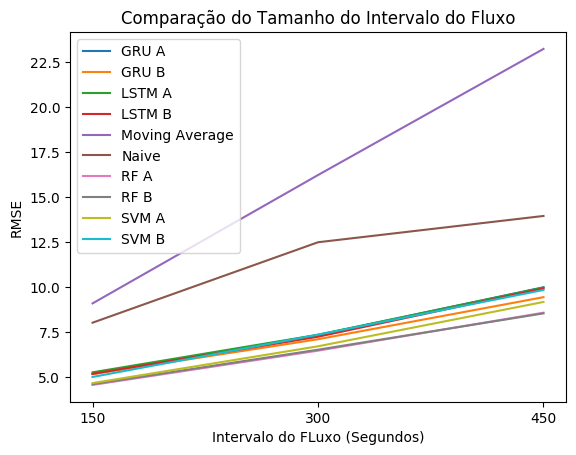
\includegraphics[scale=0.8]{monography/img/comparisons/comparacao_do_tamanho_do_intervalo_do_fluxo_rmse.png}
    \label{figure:res_flow}
    \caption{Resposta dos modelos à variação dos valores de intervalo de fluxo}
\end{figure}

\begin{table}[H]
    \begin{tabular*}{\linewidth}{@{\extracolsep{\fill}}llll}
    \toprule
     & 
    \multicolumn{1}{l}{\textbf{150}} & 
    \multicolumn{1}{l}{\textbf{300}} &
    \multicolumn{1}{l}{\textbf{450}} \\
    \midrule
    \textbf{MM} & \textbf{9.098} $\pm$ 0.740 & 16.228 $\pm$ 0.875 & 23.233 $\pm$ 1.455
    \\
    \midrule
    \textbf{Naive} & \textbf{8.026} $\pm$ 0.868 & 12.494 $\pm$ 2.059 & 13.954 $\pm$ 1.677
    \\
    \midrule
    \textbf{RF A} & \textbf{4.569} $\pm$ 0.739 & 6.472 $\pm$ 0.464 & 8.582 $\pm$ 1.416
    \\
    \midrule
    \textbf{RF B} & \textbf{4.610} $\pm$ 0.745 & 6.525 $\pm$ 0.383 & 8.543 $\pm$ 1.225
    \\
    \midrule
    \textbf{SVM A} & \textbf{4.669} $\pm$ 0.736 & 6.714 $\pm$ 0.327 & 9.178 $\pm$ 0.955
    \\
    \midrule
    \textbf{SVM B} & \textbf{5.011} $\pm$ 0.618 & 7.361 $\pm$ 0.381 & 9.843 $\pm$ 0.360
    \\
    \midrule
    \textbf{LSTM A} & \textbf{5.269} $\pm$ 0.803 & 7.356 $\pm$ 0.601 & 9.976 $\pm$ 0.802
    \\
    \midrule
    \textbf{LSTM B} & \textbf{5.188} $\pm$ 0.715 & 7.246 $\pm$ 0.631 & 9.929 $\pm$ 0.980
    \\
    \midrule
    \textbf{GRU A} & \textbf{5.183} $\pm$ 0.679 & 7.336 $\pm$ 0.602 & 9.993 $\pm$ 1.034
    \\
    \midrule
    \textbf{GRU B} & \textbf{5.164} $\pm$ 0.758 & 7.106 $\pm$ 0.663 & 9.444 $\pm$ 1.521
    \\
    \bottomrule
    \end{tabular*}
    \label{table:res_flow}
    \caption{Resultados da Comparação entre os intervalos de fluxo. Melhores resultados de cada modelo em negrito.}
\end{table}

\section{Comparação dos Resultados Otimizados}

 Por fim, foram realizados testes para otimizar os hiper-parâmetros de cada modelo e garantir as melhores predições. Para alcançar tal objetivo, foi utilizada a técnica de \textit{Grid Search} durante as comparações dos resultados das predições de curto prazo. Abaixo, na figura \ref{figure:pred_no_tuning} podem ser vistos os resultados sem \textit{Tuning} dos hiper-parâmetros e, na figura \ref{figure:pred_tuning}, com \textit{Tuning} dos hiper-parâmetros. Os valores exatos dos resultados podem ser vistos nas tabelas  \ref{table:curto_prazo_no_tuning} e \ref{table:curto_prazo_tuning}, para as predições sem e com \textit{Tuning}, respectivamente. Os valores de parâmetros utilizados para a realização deste teste foram os melhores valores encontrados nos experimentos da seção \ref{section:resultados_parametros}.

Observando a tabela \ref{table:curto_prazo_no_tuning}, é possível constatar que todos os modelos propostos pelo trabalho tiveram performance superior que os modelos utilizados como base de comparação. Dentre esses modelos propostos, o \acrlong{RF} foi o que obteve os resultados mais promissores, se mostrando o melhor modelo em todas as predições de curto prazo, seguido pelo \acrshort{SVM}. Os modelos de aprendizagem profunda apresentaram os resultados menos satisfatórios. Porém, este cenário poderia mudar caso o conjunto de dados disponível para o trabalho fosse maior, visto que modelos de aprendizagem profunda, como \acrshort{GRU} e \acrshort{LSTM}, tendem a generalizar melhor à medida que são expostos a um maior volume de dados de treinamento. 

Como dito anteriormente, o modelo que apresentou os melhores resultados foi o \acrshort{RF}. Entretanto, este cenário muda após o \textit{Tuning} dos hiper-parâmetros. Como pode ser observado na tabela \ref{table:curto_prazo_tuning}, após a otimização dos resultados, a \acrshort{SVM} passou a obter as melhores predições em todos os casos, com uma melhora de 5\% em relação aos seus resultados antes do \textit{Tuning}. Também é válido notar que todos os outros modelos também obtiveram um aumento de performance, mas não na mesma intensidade. O \acrshort{RF}, por exemplo, teve o aumento de performance menos significativo dentre todos os modelos propostos. Isso mostra que os modelos propostos possuem sensibilidades diferentes à variação de hiper-parâmetros..


%Isso mostra que determinados hiper-parâmetros podem afetar de maneira significativa a forma como os modelos realizam suas generalizações



Nos métodos de Aprendizagem profunda, ao observar a tabela \ref{table:best_hiper_deep}, pode-se notar que para os modelos que utilizam o conjunto de dados A, são necessárias menos células na rede, o que é coerente com a teoria, visto que o conjunto de dados A possui menos atributos e, consequentemente, menos informações para processar.

\begin{figure}[H]
    \centering
    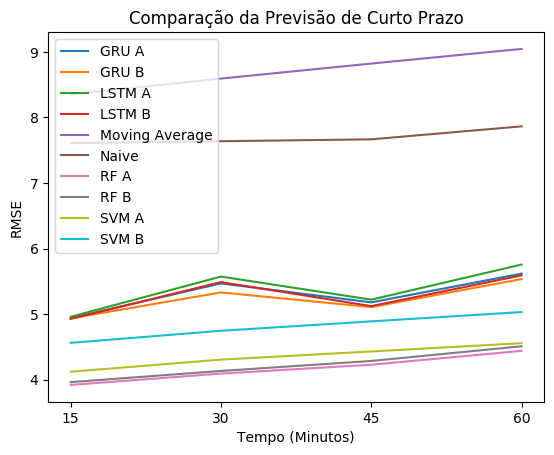
\includegraphics[scale=0.8]{monography/img/comparisons/comparacao_da_previsao_de_curto_prazo_rmse.png}
    \label{figure:pred_no_tuning}
    \caption{Comparação da previsão de curto prazo sem \textit{Tuning}}
\end{figure}

\begin{table}[H]
    \begin{tabular*}{\linewidth}{@{\extracolsep{\fill}}lllll}
    \toprule
     & 
    \multicolumn{1}{l}{\textbf{15 mins}} & 
    \multicolumn{1}{l}{\textbf{30 mins}} &
    \multicolumn{1}{l}{\textbf{45 mins}} &
    \multicolumn{1}{l}{\textbf{60 mins}} \\
\midrule
\textbf{MM} & 8.352 $\pm$ 0.820 & 8.592 $\pm$ 0.846 & 8.821 $\pm$ 0.866 & 9.044 $\pm$ 0.881
\\

\midrule
\textbf{Naive} & 7.607 $\pm$ 0.993 & 7.636 $\pm$ 0.839 & 7.665 $\pm$ 0.768 & 7.863 $\pm$ 0.889
\\

\midrule
\textbf{RF A} & \textcolor{blue}{\textbf{3.919 $\pm$ 0.395}} & \textcolor{blue}{\textbf{4.092 $\pm$ 0.409}} & \textcolor{blue}{\textbf{4.227 $\pm$ 0.467}} & \textcolor{blue}{\textbf{4.439 $\pm$ 0.513}}
\\

\midrule
\textbf{RF B} & 3.962 $\pm$ 0.400 & 4.132 $\pm$ 0.410 & 4.284 $\pm$ 0.468 & 4.508 $\pm$ 0.501
\\

\midrule
\textbf{SVM A} & 4.120 $\pm$ 0.457 & 4.305 $\pm$ 0.466 & 4.429 $\pm$ 0.491 & 4.556 $\pm$ 0.494
\\

\midrule
\textbf{SVM B} & 4.560 $\pm$ 0.465 & 4.745 $\pm$ 0.478 & 4.888 $\pm$ 0.506 & 5.030 $\pm$ 0.513
\\

\midrule
\textbf{LSTM A} & 4.958 $\pm$ 0.579 & 5.571 $\pm$ 0.539 & 5.219 $\pm$ 0.527 & 5.755 $\pm$ 0.448
\\

\midrule
\textbf{LSTM B} & 4.926 $\pm$ 0.567 & 5.487 $\pm$ 0.577 & 5.121 $\pm$ 0.582 & 5.590 $\pm$ 0.596
\\

\midrule
\textbf{GRU A} & 4.937 $\pm$ 0.579 & 5.467 $\pm$ 0.548 & 5.178 $\pm$ 0.585 & 5.616 $\pm$ 0.537
\\

\midrule
\textbf{GRU B} & 4.934 $\pm$ 0.628 & 5.330 $\pm$ 0.473 & 5.106 $\pm$ 0.619 & 5.534 $\pm$ 0.542
\\
    \bottomrule
    \end{tabular*}
    \label{table:curto_prazo_no_tuning}
    \caption{Resultados das predições de curto prazo dos modelos sem Tuning.}
\end{table}

\begin{figure}[H]
    \centering
    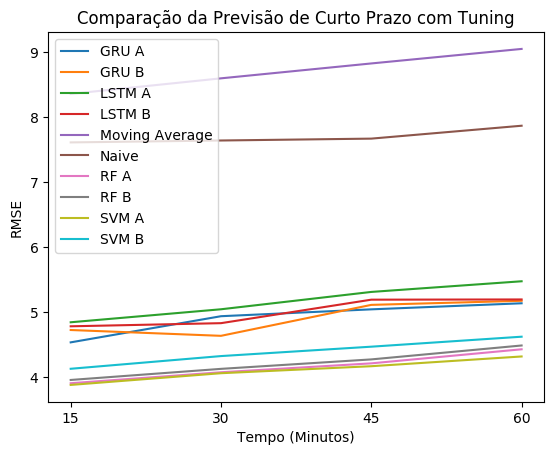
\includegraphics[scale=0.8]{monography/img/comparisons/comparacao_da_previsao_de_curto_prazo_com_tuning_rmse.png}
    \label{figure:pred_tuning}
    \caption{Comparação da previsão de curto prazo com \textit{Tuning}}
\end{figure}



\begin{table}[H]
    \begin{tabular*}{\linewidth}{@{\extracolsep{\fill}}lllll}
    \toprule
     & 
    \multicolumn{1}{l}{\textbf{15 mins}} & 
    \multicolumn{1}{l}{\textbf{30 mins}} &
    \multicolumn{1}{l}{\textbf{45 mins}} &
    \multicolumn{1}{l}{\textbf{60 mins}} \\
\midrule
\textbf{MM} & 8.352 $\pm$ 0.820 & 8.592 $\pm$ 0.846 & 8.821 $\pm$ 0.866 & 9.044 $\pm$ 0.881
\\
\midrule
\textbf{Naive} & 7.607 $\pm$ 0.993 & 7.636 $\pm$ 0.839 & 7.665 $\pm$ 0.768 & 7.863 $\pm$ 0.889
\\
\midrule
\textbf{RF A} & 3.904 $\pm$ 0.399 & 4.073 $\pm$ 0.422 & 4.210 $\pm$ 0.466 & 4.426 $\pm$ 0.512
\\
\midrule
\textbf{RF B} & 3.954 $\pm$ 0.397 & 4.125 $\pm$ 0.409 & 4.270 $\pm$ 0.474 & 4.484 $\pm$ 0.503
\\
\midrule
\textbf{SVM A} &  \textcolor{blue}{\textbf{3.878} $\pm$}  \textcolor{blue}{\textbf{0.423}} & \textcolor{blue}{\textbf{4.058 $\pm$ 0.443}} & \textcolor{blue}{\textbf{4.166 $\pm$ 0.486}} & \textcolor{blue}{\textbf{4.315 $\pm$ 0.530}}
\\
\midrule
\textbf{SVM B} & 4.126 $\pm$ 0.336 & 4.321 $\pm$ 0.384 & 4.466 $\pm$ 0.469 & 4.619 $\pm$ 0.523
\\
\midrule
\textbf{LSTM A} & 4.841 $\pm$ 0.625 & 5.041 $\pm$ 0.533 & 5.308 $\pm$ 0.379 & 5.472 $\pm$ 0.505
\\
\midrule
\textbf{LSTM B} & 4.779 $\pm$ 0.562 & 4.827 $\pm$ 0.559 & 5.189 $\pm$ 0.601 & 5.192 $\pm$ 0.691
\\
\midrule
\textbf{GRU A} & 4.532 $\pm$ 0.552 & 4.934 $\pm$ 0.306 & 5.040 $\pm$ 0.536 & 5.133 $\pm$ 0.487
\\
\midrule
\textbf{GRU B} & 4.722 $\pm$ 0.672 & 4.633 $\pm$ 0.420 & 5.109 $\pm$ 0.660 & 5.171 $\pm$ 0.537
\\
    \bottomrule
    \end{tabular*}
    \label{table:curto_prazo_tuning}
    \caption{Resultados das predições de curto prazo dos modelos com Tuning.}
\end{table}

\begin{table}[H]
    \begin{tabular*}{\linewidth}{@{\extracolsep{\fill}}lll}
    \toprule
     & 
    \multicolumn{1}{l}{\textbf{Taxa de Aprendizagem}} & 
    \multicolumn{1}{l}{\textbf{Células}} 
    \\
\midrule
\textbf{LSTM A} & 0.004 & 50\\ \midrule
\textbf{LSTM B} & 0.004 & 125 \\ \midrule
\textbf{GRU A} & 0.016 &  75 \\ \midrule
\textbf{GRU B} & 0.008 &  125 \\
    \bottomrule
    \end{tabular*}
    \label{table:best_hiper_deep}
    \caption{Valores de hiper-parâmetros mais recorrentes no Grid Search para os modelos de aprendizagem profunda.}
\end{table}

\begin{table}[H]
    \begin{tabular*}{\linewidth}{@{\extracolsep{\fill}}lll}
    \toprule
     & 
    \multicolumn{1}{l}{\textbf{C}} & 
    \multicolumn{1}{l}{\textbf{Gamma}} 
    \\
\midrule
\textbf{SVM A} & 100 & 50\\ \midrule
\textbf{SVM B} & 100 & 125 \\ \midrule

    \bottomrule
    \end{tabular*}
    \label{table:best_hiper_deep}
    \caption{Valores de hiper-parâmetros mais recorrentes no Grid Search para o SVM}
\end{table}

\begin{table}[H]
    \begin{tabular*}{\linewidth}{@{\extracolsep{\fill}}lll}
    \toprule
     & 
    \multicolumn{1}{l}{\textbf{Altura Máx. Arvore}} & 
    \multicolumn{1}{l}{\textbf{Nr. Estimadores}} 
    \\
\midrule
\textbf{RF A} & 32 & 800\\ \midrule
\textbf{RF B} & 32 & 800 \\ \midrule

    \bottomrule
    \end{tabular*}
    \label{table:best_hiper_deep}
    \caption{Valores de hiper-parâmetros mais recorrentes no Grid Search para o Random Forest.}
\end{table}

Observando os resultados da escolha de hiper-parâmetros, é perceptível que os modelos de aprendizagem profunda não precisaram de uma taxa de aprendizagem tão alta para aprender a distribuição dos dados. Porém, há uma diferença para os resultados quando os modelos utilizam o conjunto de dados A, ou B. O \acrshort{LSTM}, por exemplo, possui a mesma taxa de aprendizagem para os dois conjuntos de dados, mas a quantidade de células necessárias do conjunto B é maior, o que mostra que mesmo com uma taxa de aprendizagem igual, o conjunto de dados com maior número de informações também necessita de mais processamento para generalizar. Este padrão também se mantém com o \acrshort{GRU}, onde a taxa de aprendizagem para o modelo que utiliza o conjunto de dados B chegou a ser menor que o utilizado pelo modelo A, mas, da mesma forma que acontece com o \textit{\acrshort{LSTM}}, a quantidade de células necessárias na rede foi o dobro que o utilizado pelo modelo A.




